% Options for packages loaded elsewhere
\PassOptionsToPackage{unicode}{hyperref}
\PassOptionsToPackage{hyphens}{url}
%
\documentclass[
  english,
  man]{apa6}
\usepackage{lmodern}
\usepackage{amssymb,amsmath}
\usepackage{ifxetex,ifluatex}
\ifnum 0\ifxetex 1\fi\ifluatex 1\fi=0 % if pdftex
  \usepackage[T1]{fontenc}
  \usepackage[utf8]{inputenc}
  \usepackage{textcomp} % provide euro and other symbols
\else % if luatex or xetex
  \usepackage{unicode-math}
  \defaultfontfeatures{Scale=MatchLowercase}
  \defaultfontfeatures[\rmfamily]{Ligatures=TeX,Scale=1}
\fi
% Use upquote if available, for straight quotes in verbatim environments
\IfFileExists{upquote.sty}{\usepackage{upquote}}{}
\IfFileExists{microtype.sty}{% use microtype if available
  \usepackage[]{microtype}
  \UseMicrotypeSet[protrusion]{basicmath} % disable protrusion for tt fonts
}{}
\makeatletter
\@ifundefined{KOMAClassName}{% if non-KOMA class
  \IfFileExists{parskip.sty}{%
    \usepackage{parskip}
  }{% else
    \setlength{\parindent}{0pt}
    \setlength{\parskip}{6pt plus 2pt minus 1pt}}
}{% if KOMA class
  \KOMAoptions{parskip=half}}
\makeatother
\usepackage{xcolor}
\IfFileExists{xurl.sty}{\usepackage{xurl}}{} % add URL line breaks if available
\IfFileExists{bookmark.sty}{\usepackage{bookmark}}{\usepackage{hyperref}}
\hypersetup{
  pdftitle={Reanalysis of the Study : `For 5-Month-Old Infants, Melodies Are Social'},
  pdfauthor={Ali Haydar Ozgun1},
  pdflang={en-EN},
  hidelinks,
  pdfcreator={LaTeX via pandoc}}
\urlstyle{same} % disable monospaced font for URLs
\usepackage{graphicx,grffile}
\makeatletter
\def\maxwidth{\ifdim\Gin@nat@width>\linewidth\linewidth\else\Gin@nat@width\fi}
\def\maxheight{\ifdim\Gin@nat@height>\textheight\textheight\else\Gin@nat@height\fi}
\makeatother
% Scale images if necessary, so that they will not overflow the page
% margins by default, and it is still possible to overwrite the defaults
% using explicit options in \includegraphics[width, height, ...]{}
\setkeys{Gin}{width=\maxwidth,height=\maxheight,keepaspectratio}
% Set default figure placement to htbp
\makeatletter
\def\fps@figure{htbp}
\makeatother
\setlength{\emergencystretch}{3em} % prevent overfull lines
\providecommand{\tightlist}{%
  \setlength{\itemsep}{0pt}\setlength{\parskip}{0pt}}
\setcounter{secnumdepth}{-\maxdimen} % remove section numbering
% Make \paragraph and \subparagraph free-standing
\ifx\paragraph\undefined\else
  \let\oldparagraph\paragraph
  \renewcommand{\paragraph}[1]{\oldparagraph{#1}\mbox{}}
\fi
\ifx\subparagraph\undefined\else
  \let\oldsubparagraph\subparagraph
  \renewcommand{\subparagraph}[1]{\oldsubparagraph{#1}\mbox{}}
\fi
% Manuscript styling
\usepackage{upgreek}
\captionsetup{font=singlespacing,justification=justified}

% Table formatting
\usepackage{longtable}
\usepackage{lscape}
% \usepackage[counterclockwise]{rotating}   % Landscape page setup for large tables
\usepackage{multirow}		% Table styling
\usepackage{tabularx}		% Control Column width
\usepackage[flushleft]{threeparttable}	% Allows for three part tables with a specified notes section
\usepackage{threeparttablex}            % Lets threeparttable work with longtable

% Create new environments so endfloat can handle them
% \newenvironment{ltable}
%   {\begin{landscape}\centering\begin{threeparttable}}
%   {\end{threeparttable}\end{landscape}}
\newenvironment{lltable}{\begin{landscape}\centering\begin{ThreePartTable}}{\end{ThreePartTable}\end{landscape}}

% Enables adjusting longtable caption width to table width
% Solution found at http://golatex.de/longtable-mit-caption-so-breit-wie-die-tabelle-t15767.html
\makeatletter
\newcommand\LastLTentrywidth{1em}
\newlength\longtablewidth
\setlength{\longtablewidth}{1in}
\newcommand{\getlongtablewidth}{\begingroup \ifcsname LT@\roman{LT@tables}\endcsname \global\longtablewidth=0pt \renewcommand{\LT@entry}[2]{\global\advance\longtablewidth by ##2\relax\gdef\LastLTentrywidth{##2}}\@nameuse{LT@\roman{LT@tables}} \fi \endgroup}

% \setlength{\parindent}{0.5in}
% \setlength{\parskip}{0pt plus 0pt minus 0pt}

% \usepackage{etoolbox}
\makeatletter
\patchcmd{\HyOrg@maketitle}
  {\section{\normalfont\normalsize\abstractname}}
  {\section*{\normalfont\normalsize\abstractname}}
  {}{\typeout{Failed to patch abstract.}}
\patchcmd{\HyOrg@maketitle}
  {\section{\protect\normalfont{\@title}}}
  {\section*{\protect\normalfont{\@title}}}
  {}{\typeout{Failed to patch title.}}
\makeatother
\shorttitle{ Semester Long Project PSYC 7765/66}
\DeclareDelayedFloatFlavor{ThreePartTable}{table}
\DeclareDelayedFloatFlavor{lltable}{table}
\DeclareDelayedFloatFlavor*{longtable}{table}
\makeatletter
\renewcommand{\efloat@iwrite}[1]{\immediate\expandafter\protected@write\csname efloat@post#1\endcsname{}}
\makeatother
\usepackage{lineno}

\linenumbers
\usepackage{csquotes}
\usepackage[titles]{tocloft}
\cftpagenumbersoff{figure}
\renewcommand{\cftfigpresnum}{\itshape\figurename\enspace}
\renewcommand{\cftfigaftersnum}{.\space}
\setlength{\cftfigindent}{0pt}
\setlength{\cftafterloftitleskip}{0pt}
\settowidth{\cftfignumwidth}{Figure 10.\qquad}
\ifxetex
  % Load polyglossia as late as possible: uses bidi with RTL langages (e.g. Hebrew, Arabic)
  \usepackage{polyglossia}
  \setmainlanguage[]{english}
\else
  \usepackage[shorthands=off,main=english]{babel}
\fi

\title{Reanalysis of the Study : `For 5-Month-Old Infants, Melodies Are Social'}
\author{Ali Haydar Ozgun\textsuperscript{1}}
\date{}


\authornote{

Ali Haydar Ozgun Brooklyn College Psychology Department, Master of Art Experimental Psychology Program First Semester Student.

Correspondence concerning this article should be addressed to Ali Haydar Ozgun, 2900 Bedford Avenue. E-mail: \href{mailto:alihaydar.ozgun96@bcmail.cuny.edu}{\nolinkurl{alihaydar.ozgun96@bcmail.cuny.edu}}

}

\affiliation{\vspace{0.5cm}\textsuperscript{1} CUNY - Brooklyn College}

\abstract{
This report re-produces the analysis of Experiment 4 reported in Mehr, Song, and Spelke (2016). During a period of 1 to 2 weeks, 5-month-old babies listened to one of two new songs at home, with the same lyrics and rhythms, but different melodies; The song was either sung by a parent, came out of a toy, or was sung by an unfamiliar adult, first in person and then via video. Next, the infants' selective attention to two new people was tested after one sang the familiar song and the unfamiliar song. Infants who experienced their parents' singing looked at the new person singing the familiar tune longer than the new person singing the unfamiliar music. In this study the amount of exposure to the song at home significantly estimated the extent of this preference. And it has been shown that these listened melodies have a social feature for infants.
}



\begin{document}
\maketitle

\hypertarget{introduction}{%
\section{Introduction}\label{introduction}}

This report re-produces the analysis of Experiment 4 reported in Mehr et al. (2016). The citation for the article is:

Mehr et al. (2016) For 5-month-old infants, melodies are social. Psychological Science, 27(4), 486-501.

The data were downloaded from \url{https://osf.io/y3kzd/files/}.

Mehr et al. (2016) had 5- month old infants participants and their parent to test the infants' selective attention and social meaning of the song for infants to two novel individuals after one sang the familiar song and the other sang the unfamiliar song. Accordingly, it has been hypothesized that the songs sung for infants have a social meaning in infants. To test that, five experiments were conducted. In these experiments, infants' preferences for the speaker of a melody to be familiar or unfamiliar were examined.

In this reanalysis, the findings at the fourth experiment were analyzed, and the measurements of the infants' gaze at the familiar and unfamiliar song's toy were repeated.

\hypertarget{methods}{%
\section{Methods}\label{methods}}

\hypertarget{participants}{%
\subsection{Participants}\label{participants}}

Experiment four, tested 32 infants, but after excluding the participants who could not complete the experiment, the analyses have done on data from 22 infants. After the experiment, participants have not exposed to a familiar song and toy. Parents were asked whether they sang the song to the babies after the experiment was over.

\hypertarget{procedure}{%
\subsection{Procedure}\label{procedure}}

The Experiment contains four trials. On the trials, the experimenter was unaware of the song presented to the participants---the experimenter located a toy to one side of the infant participant. The characteristic of the trials was visually identical, and one of them played the song that they had already heard in Experiment 2 from the infant. The other one had not heard before from the participants in the Experiment. So, the infant participant listened to the familiar and unfamiliar songs twice between the trials---the infant's gaze toward the toy measured during the singing and in silence for each trial.

\hypertarget{data-analysis}{%
\subsection{Data analysis}\label{data-analysis}}

We used R (Version 4.0.3; R Core Team, 2020) and the R-packages \emph{dplyr} (Version 1.0.7; Wickham et al., 2021), \emph{ggplot2} (Version 3.3.5; Wickham, 2016), \emph{papaja} (Version 0.1.0.9997; Aust \& Barth, 2020), \emph{pwr} (Version 1.3.0; Champely, 2020), and \emph{tidyr} (Version 1.1.4; Wickham, 2021) for all our analyses.

\hypertarget{results}{%
\section{Results}\label{results}}

First, the means for Toy Playing Familiar and Unfamiliar Song collapsed across subjects in Experiment 4 are presented in Table 1.

\begin{table}[tbp]

\begin{center}
\begin{threeparttable}

\caption{\label{tab:unnamed-chunk-1}}

\begin{tabular}{lll}
\toprule
ToyPlaying & \multicolumn{1}{c}{count} & \multicolumn{1}{c}{mean}\\
\midrule
Familiar Song & 22 & 207.09\\
Unfamiliar Song & 22 & 173.73\\
\bottomrule
\end{tabular}

\end{threeparttable}
\end{center}

\end{table}

Additionally, the means for each condition are plotted in Figure 1.

\begin{figure}
\centering
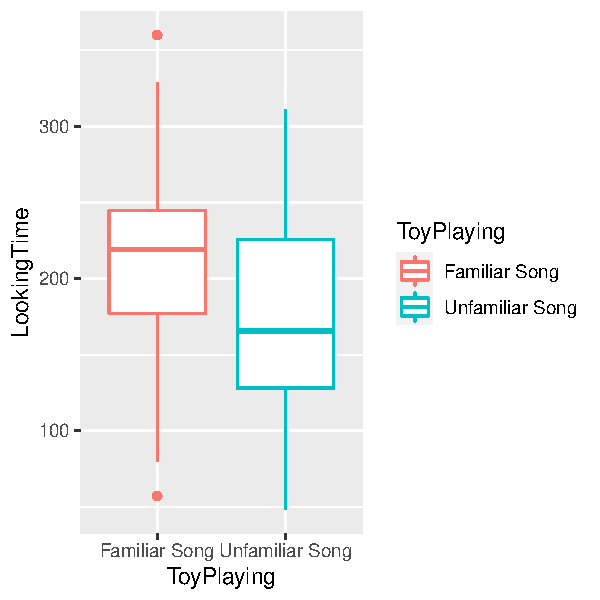
\includegraphics{SemesterProject_files/figure-latex/unnamed-chunk-2-1.pdf}
\caption{\label{fig:unnamed-chunk-2}Mean of Looking Time for Familiar and Unfamiliar Toy Playing .}
\end{figure}

The original authors reported the following in their analysis, \enquote{difference in looking time: M = 0.815 s, SD = 1.61, 95\% CI = {[}0.10, 1.53{]}), t(21) = 2.38, p = .027 (paired t test).}
Open data from this paper was obtained, and a script was generated to attempt a reproduction of the analysis. The following results are generated by the R analysis script.

The re-analysis for the differences between familiar and unfamiliar toy playing songs showed, \(M_d = 24.45\), 95\% CI \([3.04\), \(45.87]\), \(t(21) = 2.38\), \(p = .027\).

\hypertarget{power-analysis}{%
\section{Power Analysis}\label{power-analysis}}

The following reports a power curve analysis for the t-tests in the design. This shows the power of the design to detect effects of different sizes.

\begin{figure}
\centering
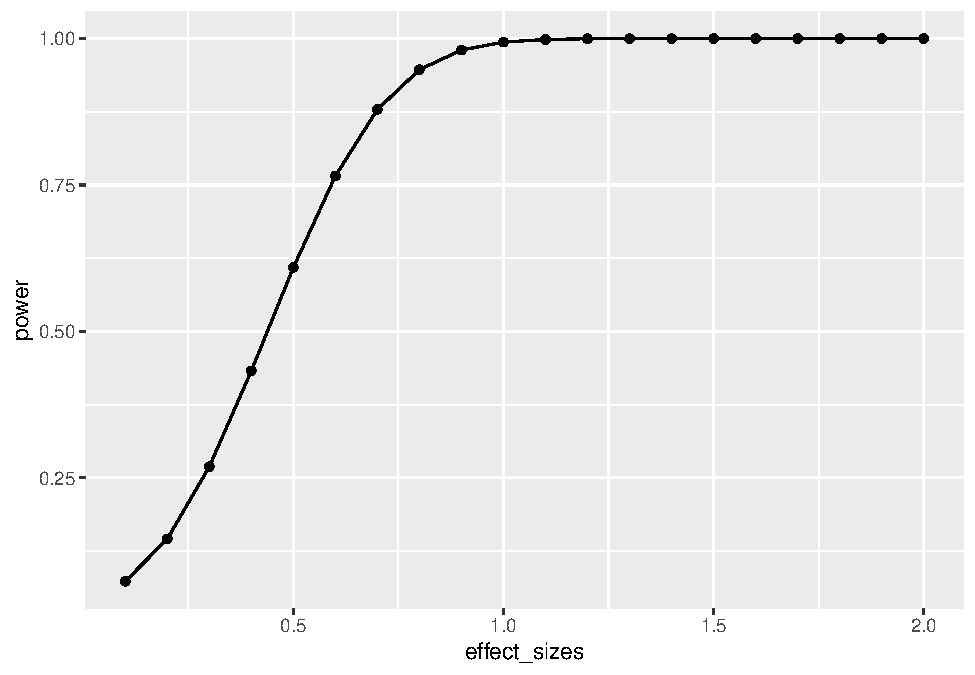
\includegraphics{SemesterProject_files/figure-latex/unnamed-chunk-4-1.pdf}
\caption{\label{fig:unnamed-chunk-4}A power curve analysis for a paired sample t-test with 22 participants.}
\end{figure}

\hypertarget{discussion}{%
\section{Discussion}\label{discussion}}

Experiment 4 results show that infants can distinguish between familiar and unfamiliar songs. In other words, experimental findings from Experiment 4 show that when babies hear familiar songs, they tend to look longer at the toy from which the familiar song comes.

\newpage

\hypertarget{references}{%
\section{References}\label{references}}

\begingroup
\setlength{\parindent}{-0.5in}
\setlength{\leftskip}{0.5in}

\hypertarget{refs}{}
\leavevmode\hypertarget{ref-R-papaja}{}%
Aust, F., \& Barth, M. (2020). \emph{papaja: Create APA manuscripts with R Markdown}. Retrieved from \url{https://github.com/crsh/papaja}

\leavevmode\hypertarget{ref-R-pwr}{}%
Champely, S. (2020). \emph{Pwr: Basic functions for power analysis}. Retrieved from \url{https://CRAN.R-project.org/package=pwr}

\leavevmode\hypertarget{ref-mehr2016}{}%
Mehr, S. A., Song, L. A., \& Spelke, E. S. (2016). For 5-month-old infants, melodies are social. \emph{Psychological Science}, \emph{27}(4), 486--501.

\leavevmode\hypertarget{ref-R-base}{}%
R Core Team. (2020). \emph{R: A language and environment for statistical computing}. Vienna, Austria: R Foundation for Statistical Computing. Retrieved from \url{https://www.R-project.org/}

\leavevmode\hypertarget{ref-R-ggplot2}{}%
Wickham, H. (2016). \emph{Ggplot2: Elegant graphics for data analysis}. Springer-Verlag New York. Retrieved from \url{https://ggplot2.tidyverse.org}

\leavevmode\hypertarget{ref-R-tidyr}{}%
Wickham, H. (2021). \emph{Tidyr: Tidy messy data}. Retrieved from \url{https://CRAN.R-project.org/package=tidyr}

\leavevmode\hypertarget{ref-R-dplyr}{}%
Wickham, H., François, R., Henry, L., \& Müller, K. (2021). \emph{Dplyr: A grammar of data manipulation}. Retrieved from \url{https://CRAN.R-project.org/package=dplyr}

\endgroup


\clearpage
\renewcommand{\listfigurename}{Figure captions}


\end{document}
